\title{A comparison between genome-wide and per-gene tri-nucleotide distributions}
\author{Romain Strock}
\date{\today}

\documentclass[12pt]{article}
\usepackage{amsmath}
\usepackage{mathrsfs}
\usepackage{graphicx}
\usepackage{booktabs}
\usepackage[svgnames,table]{xcolor}
\usepackage{pifont}
\usepackage{hyperref}

\graphicspath{ {./diagrams/} }

\begin{document}
\maketitle

\begin{abstract}
I computed the genome-wide and per-gene tri-nucleotide distributions of 20,000 strains of bacterial and archaeal species. Genes were further decomposed into protein domains from Pfam \& TIGR. I seeked to understand whether certain domains had distributions consistently similar - or conversely dissimilar - to their genome mean distribution. A handful of domains have a distribution systematically close to the mean, the strongest evidence of which are for tRNA synthetase domains such as ``tRNA synt 1''. On the other hand, distributions of domains related to ribosome structure such as ``Ribosomal L23'' are shown to be consistently different to their genome-wide mean. In both cases, most top domains appear related to translational activities.
\end{abstract}

\section{Goal}
We are looking to find out whether certain protein domains have a distribution of tri-nucleotides consistently close to their genome-wide tri-nucleotide distribution across a dataset of 20,000-odd strains of prokaryotes.

\section{Method}

\paragraph{Genomes}
A dataset of 19,741 strains from 19,228 species was selected, including 18,322 bacterial strains \& 1,419 archaeal strains. Sequences \& annotations were retrieved from GenBank~\cite{benson2012genbank}. When missing, annotations were predicted with Prodigal~\cite{hyatt2010prodigal}. Selection \& processing by courtesy of Antoine.

\paragraph{Protein domains}
A dataset of protein domains from Pfam~\cite{bateman2004pfam} \& TIGRFAM~\cite{haft2003tigrfams} was retrieved and aligned against all of the 20,000 genomes, once again courtesy of Antoine.

\paragraph{Tri-nucleotide distributions}
Distribution of tri-nucleotides is computed by counting triplets of nucleotides on a set of DNA sequences and their reverse complements, then dividing each value by the sum of all triplet counts.

\paragraph{Genome-wide \& per-gene distributions}
Specifically, genome-wide distributions are computed by considering all chromosome \& plasmid sequences of a given strain as well as their reverse complements. Similarly, per-gene distributions are computed by considering triplets from CDS and their reverse complements, i.e. disregarding reading frames.

\paragraph{Comparing distributions}
Information theory provides mechanisms to measure the similarity between probability distributions; one such method is the \textit{Kullback–Leibler divergence}~\cite{kullback1951information}, defined as follow for two distributions P and Q defined on probability space $X$:
%
\begin{equation}
D_{KL}(P, Q) = \sum\limits_{x \in X} P(x) (\log_2 P(x) - \log_2 Q(x))
\end{equation}
%
Notice that KL divergence is asymmetric, i.e. $D_{KL}(P, Q) \neq D_{KL}(Q, P)$. More concernedly, the KL divergence has no upper bound. An easier metric to work with is the \textit{Jensen-Shannon distance}~\cite{fuglede2004jensen}, which is based on the KL divergence but is symmetric and bounded on $[0, 1]$:
%
\begin{equation}
\begin{split}
JSD(P, Q) &= \sqrt{\frac{1}{2}D_{KL}(P, M) + \frac{1}{2}D_{KL}(Q, M)} \\
\\
& where \; M = \frac{1}{2}(P + Q)
\end{split}
\end{equation}
%
Example: the distribution of distances between E.~coli's gene distributions and its genome-wide distribution -- along with the distance to two other genome-wide distributions -- are shown in figure~\ref{fig:e_coli_distances}.

\pagebreak

\begin{figure}[!htb]
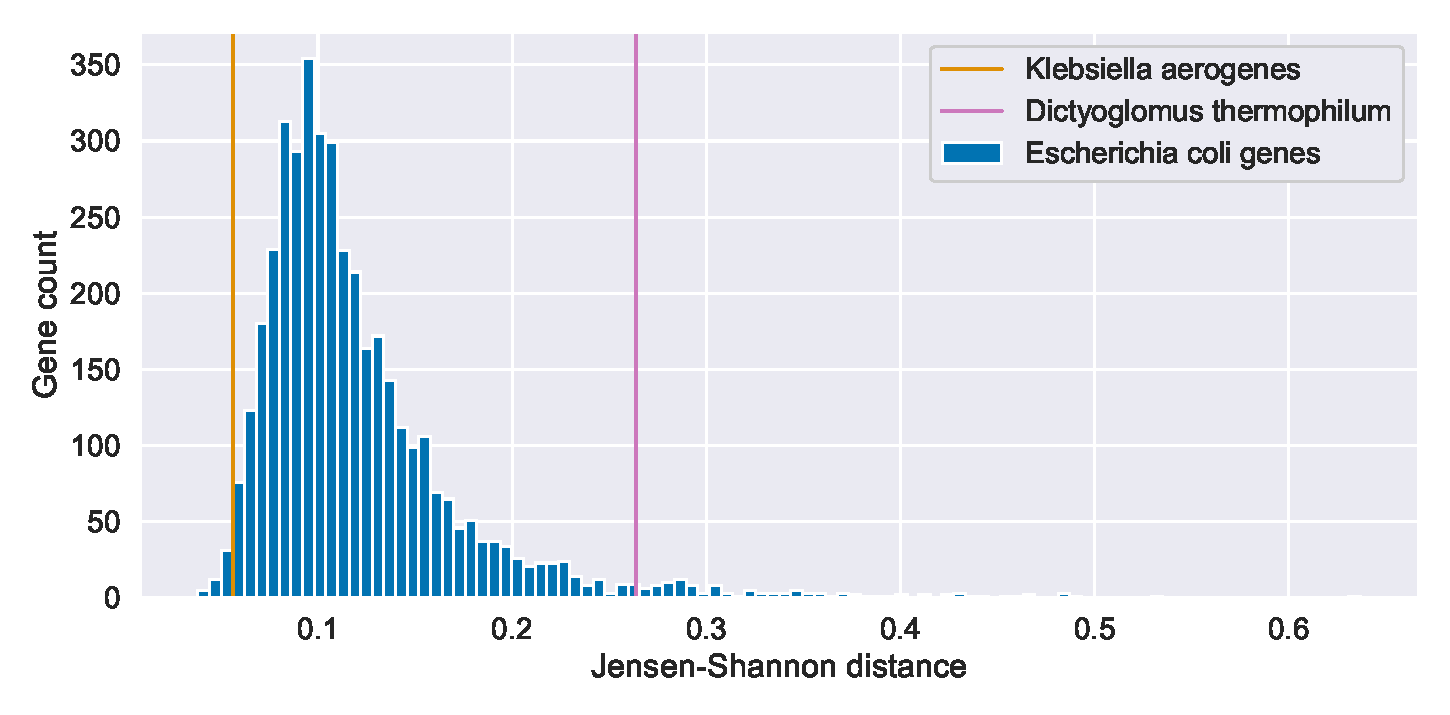
\includegraphics[scale = .55]{e_coli_distances.eps}
\caption{Distribution of Jensen-Shannon distances between the genome-wide tri-nucleotide distribution of \textit{E.~coli K-12} and all of its individual genes. Orange line: \textit{Klebsiella aerogenes} genome-wide (same family as \textit{E.~coli}).\\Pink line: \textit{Dictyoglomus thermophilum} genome-wide (different phylum).}
\label{fig:e_coli_distances}
\end{figure}

\paragraph{Probability of closeness: genes}
To achieve our stated goal, we ought to assign likeliness to events such as ``Protein domain PAS is consistently near the genome-wide tri-nucleotide distributions at aggregation level $L$'' where $L$ could be ``assembly'', ``phylum'' or ``overall'' for example.\\
\\
For a given assembly, a protein domain may be present in several genes, e.g. 11 times for Pfam domain ``PAS'' in \textit{E.~coli K-12}. Thus, let's first define the probability for gene $g$ of having a tri-nucleotide distribution close to its genome-wide distribution:

\begin{description}
	\item $D_a$ is the genome-wide tri-nucleotide distribution for assembly $a$.
	\item $D_{a,g}$ is the tri-nucleotide distribution for gene $g$ in assembly $a$.  
	\item $D_{a,g} \mid\mid D_a$ is the event ``$D_{a,g}$ is close to the genome-wide distribution $D_a$''.
	\item $P(D_{a,g} \mid\mid D_a)$ is the probability of event $D_{a,g} \mid\mid D_a$, defined as follows:
\end{description}
%
\begin{equation}
P(D_{a,g} \mid\mid D_a) = 1 - JSD(D_{a,g}, D_a)
\end{equation}
%
When $D_a$ and $D_{a,g}$ are close, the Jensen-Shannon distance is near 0, therefore the probability is close to 1, and vice versa.\\
\\
It follows that event $\overline{D_{a,g} \mid\mid D_a}$ -- the negation of $D_{a,g} \mid\mid D_a$, representing the statement ``$D_{a,g}$ is far from the genome-wide distribution $D_a$'' -- has probability:

\begin{equation}
P(\overline{D_{a,g} \mid\mid D_a}) = 1 - P(D_{a,g} \mid\mid D_a) = JSD(D_{a,g}, D_a)
\end{equation}

\paragraph{Probability of closeness: domains}
Equipped with the formalism presented previously, we can turn to defining the likeliness of a protein domain being consistently close to the genome-wide distribution:\\
\\
$G_{a, \delta}$ is the set of genes in assembly $a$ containing protein domain $\delta$.\\
\\
$\mathscr{E_{\delta}} \mid a$ is the event ``Protein domain $\delta$ is consistently near the genome-wide tri-nucleotide distributions at assembly level'', defined as:
%
\begin{equation}
\mathscr{E_{\delta}} \mid a = \bigcap\limits_{g \in G_{a, \delta}} D_{a,g} \mid\mid D_a
\end{equation}
%
That is, $\mathscr{E_{\delta}} \mid a$ is the intersection of events $D_{a,g} \mid\mid D_a$, $\forall g \in G_{a, \delta}$.\\
\\
Assuming that events $D_{a,g} \mid\mid D_a$ are independent from each others when conditioning on $a$, it follows~\cite{dupre2009new} that $P(\mathscr{E_{\delta}} \mid a)$ is defined as:
%
\begin{equation}
P(\mathscr{E_{\delta}} \mid a) = \prod\limits_{g \in G_{a, \delta}} P(D_{a,g} \mid\mid D_a)
\label{eq:assembly_probability}
\end{equation}

\paragraph{Phylum aggregation}
Similarly, for each phylum $\phi$, we can define the event $\mathscr{E_{\delta}} \mid \phi$ as ``Protein domain $\delta$ is consistently near the genome-wide tri-nucleotide distributions at phylum level''. Assuming that genomes are independent from each other when conditioning on their phylum $\phi$, we get:
%
\begin{equation}
P(\mathscr{E_{\delta}} \mid \phi) = \prod\limits_{a \in \phi} P(\mathscr{E_{\delta}} \mid a)
\label{eq:phylum_probability}
\end{equation}
%
Probabilities for other phylogenetic events such as class, family or genus can be derived in much the same way.

\paragraph{Overall aggregation}
Lastly, we want to aggregate protein domain events at superkingdom or even prokaryotic level. Extra care must be taken to avoid biases due to evolutionary history: we ought to control for the phylogeny.\\
\\
One common way~\cite{greenland1999confounding} to do so is to compute probabilities separately for each phylum using equation~\ref{eq:phylum_probability}, before aggregating values in a weighted sum:
%
\begin{equation}
P(\mathscr{E_{\delta}}) = \sum\limits_{\phi} P(\mathscr{E_{\delta}} \mid \phi)P(\phi)
\label{eq:overall_probability}
\end{equation}
%
The term $P(\phi)$, often called \textit{prior probability}, can be used to weight phyla differently. In the following, we'll assume that each phylum has the same weight, i.e. equation~\ref{eq:overall_probability} simplifies to the mean over $P(\mathscr{E_{\delta}} \mid \phi)$ for all $\phi$.

\paragraph{Null hypothesis}
With equation~\ref{eq:overall_probability}, we have defined a way to quantify the likeliness of expression ``Protein domain $\delta$ is consistently near its genome-wide tri-nucleotide distributions''. What's left is to define what qualifies as a large enough probability versus statistical noise: we want to compare these values against a relevant baseline.\\
\\
We wish to define the probability $P_{null}(\cdot)$, before comparing it against the actual likeliness computed previously. All we have to do is to assign a probability to the event $D_{a,g} \mid\mid D_a$ for the null hypothesis. All other probabilities can be computed with equations~\ref{eq:assembly_probability}, \ref{eq:phylum_probability} and \ref{eq:overall_probability}.\\
\\
A simple way to define $P_{null}(D_{a,g} \mid\mid D_a)$ is to set it to the mean of $P(D_{a,g}~\mid\mid~D_a)$:
%
\begin{equation}
P_{null}(D_{a,g} \mid\mid D_a) = \frac{1}{N}\sum\limits_{g^{\prime}=1}^{N} P(D_{a,g^{\prime}} \mid\mid D_a)
\end{equation}
%
Note that all genes in an assembly get the same ``null value''.\\
\\
If a protein domain $\delta$ is consistently higher than the mean, then it's a sign that we might have found an interesting domain. On the other end, if the protein domain is always lower than the mean, or is alternating, then we can easily discard it. Figure~\ref{fig:trna_synt_1g_dist} shows an example for domain ``tRNA Synt 1g''.

\pagebreak

\begin{figure}[!htb]
\hspace*{-1.2cm}
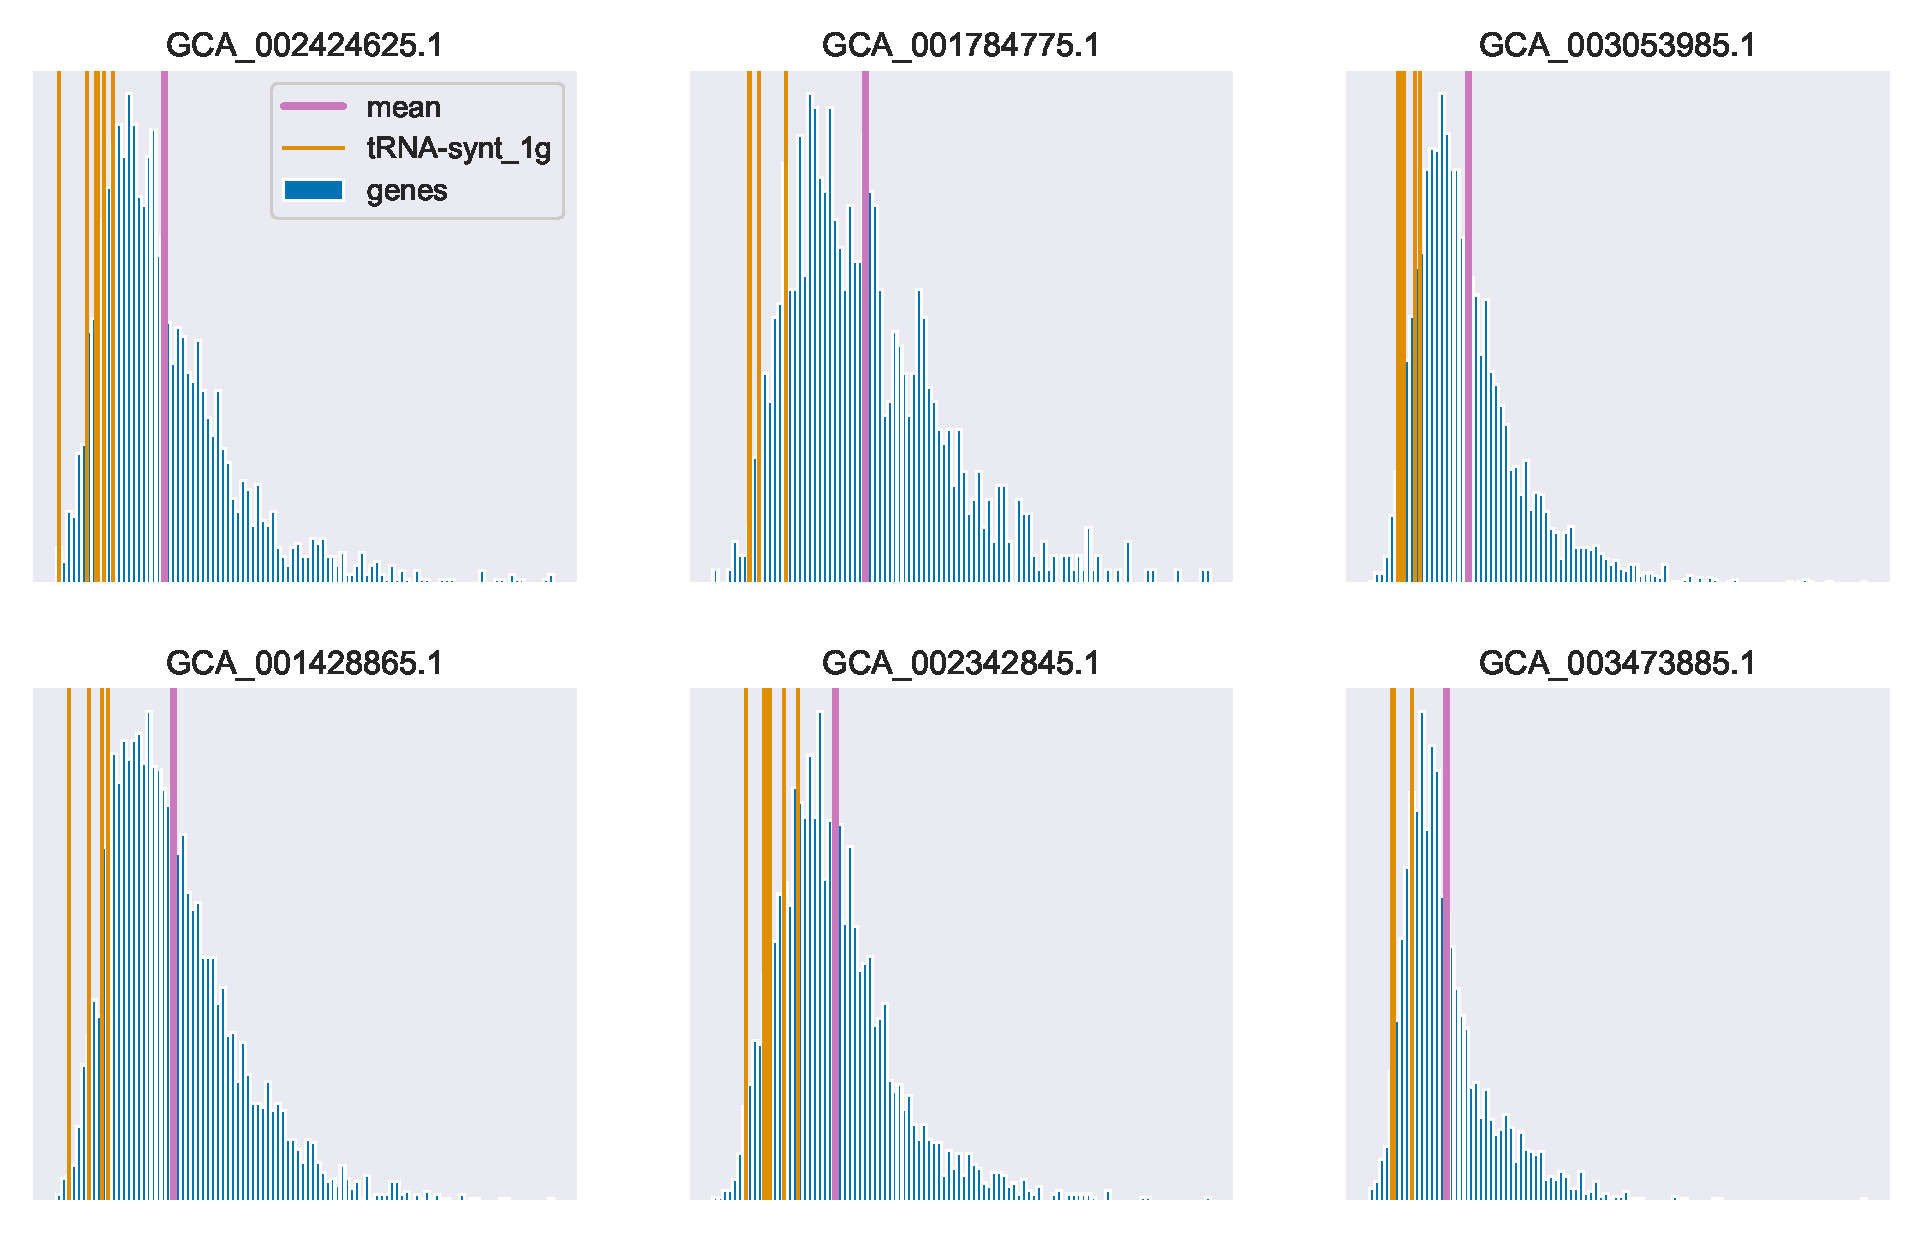
\includegraphics[scale = .5]{trna_synt_1g_dist.eps}
\caption{Null hypothesis (pink) versus actual distances of Pfam domain ``tRNA Synt 1g'' (orange) for a random selection of 6 assemblies. This domain consistently ``beats'' the null hyphotesis.}
\label{fig:trna_synt_1g_dist}
\end{figure}

\paragraph{Evidence}
The strength of evidence for a given protein domain $\delta$ is simply the ratio between actual and ``null'' probabilitites, a quantity often referred to as \textit{Bayes factor}~\cite{kass1995bayes}:
%
\begin{equation}
K_{\delta} = \frac{P(\mathscr{E_{\delta}})}{P_{null}(\mathscr{E_{\delta}})}
\end{equation}
%
\\
Evidence is customary measured in $log_{10}\,K_{\delta}$.\\ 
A common scale of interpretation is given in table~\ref{table:evidence}.

\pagebreak

\begin{table}
	\centering
    \rowcolors{2}{}{gray!10}
    \begin{tabular}{c c l}
        \toprule
        $log_{10}\,K_{\delta}$ & $K_{\delta}$ & Evidence \\
        \midrule
        $<$ 0 & $<$ 1 & Negative \\
        0 to 0.5 & 1 to 3 & Weak \\
        0.5 to 1 & 3 to 10 & Substantial \\
        1 to 1.5 & 10 to 30 & Strong \\
        1.5 to 2 & 30 to 100 & Very Strong \\
        $>$ 2 & $>$ 100 & Decisive \\
        \bottomrule
    \end{tabular}
    \caption{Strength of evidence}
    \label{table:evidence}
\end{table}

\section{Results}

\paragraph{Pfam}
Tables \ref{table:pfam_left_overall} and \ref{table:pfam_right_overall} provide a list of Pfam domains with substantial evidence for events $\mathscr{E_{\delta}}$ (close to the mean) and $\overline{\mathscr{E_{\delta}}}$ (far from the mean).

\begin{table}[!h]
	\centering
	\hspace*{-1.2cm}
    \rowcolors{2}{}{gray!10}
    \begin{tabular}{l l c l}
        \toprule
        Domain $\delta$ & Description & $log_{10}\,K_{\delta}$ & Evidence \\
        \midrule
        tRNA synt 1g & tRNA synthetases class I (M) & 1.3 & Strong \\
        tRNA synt 1 & tRNA synthetases class I (I, L, M, V) & 1.2 & Strong \\
        AAA & ATPase family & 1.1 & Strong \\
        Anticodon 1 & Anticodon-binding domain of tRNA ligase & 0.9 & Substantial \\
        tRNA synt 2b & tRNA synthetase class II (G, H, P, S, T) & 0.8 & Substantial \\
        MMR HSR1 & 50S ribosome-binding GTPase & 0.8 & Substantial \\
        HGTP anticodon & Anticodon binding domain & 0.7 & Substantial \\
        ABC tran & ABC transporter & 0.7 & Substantial \\
        tRNA anti codon & OB-fold nucleic acid binding domain & 0.7 & Substantial \\
        ResIII & Type III restriction enzyme, res subunit & 0.7 & Substantial \\
        AAA 21 & Putative AbiEii toxin, Type IV TA system & 0.6 & Substantial \\
        GTP EFTU & Elongation factor Tu GTP binding domain & 0.6 & Substantial \\
        tRNA synt 1e & tRNA synthetases class I (C) & 0.6 & Substantial \\
        Helicase C & Helicase conserved C-terminal domain & 0.6 & Substantial \\
        tRNA synt 2 & tRNA synthetases class II (D, K, N) & 0.6 & Substantial \\
        \bottomrule
    \end{tabular}
    \caption{Pfam domains consistently \textit{close} to the mean (substantial or higher)}
    \label{table:pfam_left_overall}
\end{table}

\begin{table}[!h]
	\centering
	\hspace*{-1.2cm}
    \rowcolors{2}{}{gray!10}
    \begin{tabular}{l l c l}
        \toprule
        Domain $\delta$ & Description & $log_{10}\,\overline{K_{\delta}}$ & Evidence \\
        \midrule
        eIF-1a & Translation initiation factor IF-1 & 1.6 & Very Strong \\
        Ribosomal L23 & Ribosomal protein L23 & 1.1 & Strong \\
        HTH 11 & HTH domain & 1.0 & Strong \\
        SecE & Subunits of protein translocation complex & 1.0 & Strong \\
        Ribosomal S17 & Ribosomal protein S17 & 0.9 & Substantial \\
        Ribosomal S10 & Ribosomal protein S10p / S20e & 0.9 & Substantial \\
        Ribosomal S15 & Ribosomal protein S15 & 0.8 & Substantial \\
        KOW & KOW Motif & 0.8 & Substantial \\
        Ribosomal L27A & Ribosomal proteins 50S-L15 & 0.7 & Substantial \\
        Ribosomal S19 & Ribosomal protein S19 & 0.7 & Substantial \\
        Ribosomal L29 & Ribosomal protein L29 protein & 0.7 & Substantial \\
        Ribosomal L11 & Ribosomal L11, RNA binding domain & 0.6 & Substantial \\
        DUF87 & Helicase HerA, central domain & 0.6 & Substantial \\
        Ribosomal L10 & Ribosomal protein L10 & 0.6 & Substantial \\
        \bottomrule
    \end{tabular}
    \caption{Pfam domains consistently \textit{far} from the mean (substantial or higher)}
    \label{table:pfam_right_overall}
\end{table}

\pagebreak

\paragraph{TIGRFAM}
A single TIGR domain with substantial evidence or higher is showing up for both events $\mathscr{E_{\delta}}$ and $\overline{\mathscr{E_{\delta}}}$:
%
\begin{itemize}
  \item Close to the mean: Small GTP-binding protein domain (TIGR00231).
  \item Far from the mean: Ribosomal protein L29 (TIGR00012).
\end{itemize}
%
It's worth mentioning that the next top results for $\mathscr{E_{\delta}}$ are a litany of tRNA ligase domains, although all of them have weak stength of evidence. Similarly, there are some more ribosomal proteins in the next top results for $\overline{\mathscr{E_{\delta}}}$.\\
\\
More granular results are also available at superkingdom and phylum level and show very similar trend, usually with a larger set of substantial domains.

\pagebreak

\section{Discussion}

We set out to determine whether certain protein domains have a distribution of tri-nucleotides consistently close to (or far from) their genome-wide distribution. Our results seem to suggest that a handful of proteins actually do.\\
\\
Interestingly, most protein domains in both tails of the distribution (close and far from the genome mean) appear related to translational activities, suggesting that we may be observing a single mechanism at play.\\
\\
That being said, we know that domains close to the mean have a distribution dependent on their assembly (by definition), but we cannot say the same for "far away" domains: perhaps all the ribosomal proteins are far from their genome-wide mean because they all are similar in composition, notwithstanding their assembly or phylum - something we could easily verify.\\
\\
Our analysis so far has been focusing on \textit{if}, not \textit{why} such patterns exist.\\
\\
Our approach using a null hypothesis as a baseline for comparison should have normalized any irrelevant differences between domains, such as how many times they appear in a genome, or whether or not they appear within short or long sequences. However, it would be good to double check if there is a correlation between top results and gene expression. I've checked so on the previous smaller dataset, and it wasn't the case, but I'll check again.\\
\\
If these simple sanity checks come back negative, then what could be causing these conserved tri-nucleotide distributions to occur?\\
\\
Antoine suggested it may have something to do with \textit{expression robustness}: all of these domains are bottlenecks to the creation of other proteins, so it could be that such tri-nucleotide disstribution makes their identification seamless. What experiment could we derive to test that hypothesis?

\pagebreak

\bibliographystyle{abbrv}
\bibliography{tri_nucleotide_dist}

\end{document}
